\documentclass[a4paper,oneside,DIV=12,12pt]{scrartcl}

\usepackage{graphicx}
\usepackage{float}

\usepackage{fontspec}
\setmainfont{STIX Two Text}
%\setsansfont{Roboto}
\newfontfamily{\cyrillicfontsf}{Roboto}

\usepackage{microtype}

\usepackage{polyglossia}
\setmainlanguage{ukrainian}

%%% Math typesetiing
\usepackage{amsmath}
\usepackage{unicode-math}
\setmathfont{STIX Two Math}
\usepackage[retainorgcmds]{IEEEtrantools}
\DeclareMathOperator{\tg}{tg}
%%%

\usepackage{booktabs}
\usepackage{longtable}

%%% SI units typesetiing
\usepackage{siunitx}
\sisetup{output-decimal-marker = {,},
exponent-product = {\cdot}}
\DeclareSIUnit \voltampere { ВА }
\DeclareSIUnit \var        { вар }
%%%

%%% Tikz
\usepackage{tikz}
\usepackage{tikzscale}
\usetikzlibrary{calc}
\usetikzlibrary{arrows.meta}
\usetikzlibrary{angles}
\usetikzlibrary{quotes}
\usetikzlibrary{datavisualization}

\usepackage{pgfplots}
\pgfplotsset{compat=1.15}
%%%

%%% Captions, subcaptions and subfloats
\usepackage{caption}
\usepackage{subcaption}
\captionsetup[subfigure]{labelformat=simple, labelformat=brace}
%%%

\newcommand\schel[1]{\textit{#1}}

\begin{document}
	\begin{titlepage}
		\begin{center}
			Міністерство освіти і науки України\\
			Національний авіаційний університет\\
			Навчально-науковий інститут комп'ютерних інформаційних технологій\\
			Кафедра комп'ютеризованих систем управління
			
			\vspace{\fill}
				Лабораторна робота №3\\
				з дисципліни «Теорія електричних та магнітних кіл»\\
				на тему: «Дослідження нерозгалуженого \\
				електричного~кола синусоїдного~струму»\\
				% Варіант №
				
			\vspace{\fill}
			
			\begin{flushright}
				Виконав:\\
				студент ННІКІТ СП-225\\
				Клокун Владислав\\
				Перевірив:\\
				Молчанов О.~В.
			\end{flushright}
			Київ 2017
		\end{center}
	\end{titlepage}
	
	\section{Мета роботи}
		\begin{enumerate}
			\item Використовуючи вимірювальні прилади, набути навички визначення параметрів ланцюга змінного струму, а саме: активного опору резистора, активного і реактивного опорів реальної котушки індуктивності і реального конденсатора.
			\item Дослідити різні комбінації послідовного включення в ланцюг активного резистора, котушки індуктивності і конденсатора.
			\item Дослідити резонанс у послідовному контурі.
		\end{enumerate}
		
	\section{Короткі теоретичні відомості}
		Для того, щоб визначити значення опорів різних елементів електричних ланцюгів, необхідно виміряти за допомогою приладів значення напруги, прикладеної до елемента, значення струму, який по ньому протікає, а також активну потужність, що виділяється, та кут зсуву фази. Ці величини вимірюються за допомогою вольтметра, амперметра, ватметра, фазометра.
		
		Значення активного опору резистора визначається за законом Ома:
		\[
			R = \frac{U}{I}.
		\]
		
		Потужність, споживана елементом, виділяється у вигляді тепла тільки на активних резисторах і вимірюється ватметром. Тому опір активного резистора можна визначити ще й за формулою:
		\[
			R = \frac{P}{I^2}.
		\]
		
		Щоб визначити значення активного опору реальних котушки індуктивності і конденсатора за допомогою вольтметра, амперметра і ватметра, використовуємо формули, що отримуємо з трикутника опорів:
		\[
			Z = \sqrt{R^2 + X^2},
		\]
		де $Z = \frac{U}{I}$ --- модуль повного опору кола (\si{\ohm}), $R$ --- повний активний опір кола (\si{\ohm}), $X$ --- повний реактивний опір кола (\si{\ohm}), $U$ --- діюче значення синусоїдної напруги (\si{\volt}), $I$ --- діюче значення синусоїдного струму (\si{\ampere}).
		
		\[
			X = X_K - X_C = \omega L - \frac{1}{LC},
		\]
		де $X_K$ --- реактивний індуктивний опір кола (\si{\ohm}), $X_C$ --- реактивний ємністний опір кола (\si{\ohm}), $L$ --- індуктивність котушок кола (\si{\henry}), $C$ --- ємність конденсаторів кола {\si{\farad}}, $\omega$ --- кутова частота (\si{\radian\per\second}).
		
		\[
			\omega = 2 \pi f,
		\]
		$f$ --- циклічна частота (\si{\hertz}).
		
	\section{Порядок виконання роботи}
		Зібрати вимірювальну частину схеми (рис.~\ref{fig:schematic}), використовуючи амперметр, фазометр, мультиметр і, підключаючи по черзі (лабораторний блок №8) резистор, котушку індуктивності і конденсатор, зробити необхідні вимірювання і занести їх в табл.~\ref{tab:measurements1}. 
		
		\begin{figure}[!htbp]
		\centering
			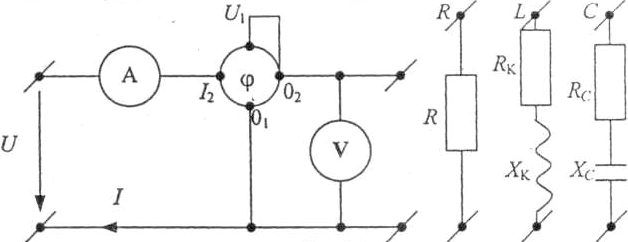
\includegraphics[height = 6\baselineskip]{assets/schematic.png}
		\caption{Вимірювальна частина схеми}
		\label{fig:schematic}
		\end{figure}
		
		\begin{longtable}[c]{
			l
			S[table-format=2.1]
			S[table-format=3e1]
			S[table-format=2]
			S[table-format=2.1]
			S[table-format=2.1]
			S[table-format=2.1]
			S[table-format=1.2]
			S[table-format=1.2]
			S[table-format=1.2]
			S[table-format=1.2]
			S[table-format=2.2]
		}
			\toprule
				{Коло} & \multicolumn{6}{c}{Виміряти} & \multicolumn{5}{c}{Обчислити опір, \si{\ohm}} \\
				\cmidrule(lr){2-7} \cmidrule(lr){8-12}
				& {$U, \si{\volt}$} & {$I, \si{\ampere}$} & {$\varphi, \si{\degree}$} & {$U_R, \si{\volt}$} & {$U_K, \si{\volt}$} & {$U_C, \si{\volt}$} & {$R$} & {$R_{K}$} & {$R_C$} & {$X_K$} & {$X_C$} \\
			\midrule
			\endhead
			\bottomrule
			\caption{Вимірювання 1}
			\endfoot
			\label{tab:measurements1}
			
				R & 10.1 & 157e-3 & 0  & 10.1 & {—}  & {—}  & 0.06 & {—}  & {—}  & {—} & {—} \\
				L & 11.0 &  76e-3 & 77 & {—}  & 11.1 & {—}  & {—}  & 0.14 & {—}  & {*} & {—} \\
				C & 11.3 &  62e-3 & 90 & {—}  & {—}  & 11.3 & {—}  & {—}  & 0.18 & {—} & {—} \\
		\end{longtable}
		
		Використовуючи виміряні величини, обчислити значення активного опору резистора, активного і реактивного опорів котушки індуктивності і конденсатора. Отримані значення занести в табл.~\ref{tab:measurements1}.
		
		Підключаючи послідовно до вимірювальної частини схеми комбінації елементів \schel{RL}, \schel{RC}, \schel{RLC}, зробити необхідні вимірювання та занести їх в табл.~\ref{tab:measurements2}.
		
		\begin{longtable}[c]{
			l
			S[table-format=2.1]
			S[table-format=2e1]
			S[table-format=+2, retain-explicit-plus]  % FIXME: show plus sign too
			S[table-format=1.1]
			S[table-format=1.1]
			S[table-format=1.1]
			S[table-format=1.1]
			S[table-format=2.1]
		}
			\toprule
				{Коло} & {$U, \si{\volt}$} & {$I, \si{\ampere}$} & {$\varphi, \si{\degree}$} & {$U_R, \si{\volt}$} & {$U_K, \si{\volt}$} & {$U_C, \si{\volt}$} & {$U_R + U_K, \si{\volt}$} & {$U_R + U_C, \si{\volt}$} \\
			\midrule
			\endhead
			\bottomrule
			\caption{Вимірювання 2}
			\endfoot
			\label{tab:measurements2}
			
				\schel{RL}  & 10.9 & 39e-3 & +33 & 7.7 & 6.2 & {—} & {—} & {—} \\
				\schel{RC}  & 10.9 & 28e-3 & -34 & 8.8 & {—} & 6.4 & {—} & {—} \\
				\schel{RLC} & 10.8 & 31e-3 & -9  & 9.5 & 5.2 & 6.9 & 5.3 & 11.8\\
		\end{longtable}
		
		Підключити до вимірювальної частини схеми тільки котушку індуктивності (лабораторний блок №8) і конденсатор (магазин ємності). Знаючи величину реактивного опору котушки, визначити значення резонансної ємності, встановити на вході схеми напругу \SIrange[range-phrase = --]{5}{7}{\volt} і, змінюючи ємність конденсатора у діапазоні \SIrange[range-phrase = --]{0}{99,5}{\micro\farad}, виміряти величини, вказані в табл.~\ref{tab:measurements3}.
		
		\begin{longtable}[c]{
			l
			S[table-format = 2.1]
			S[table-format = 3.1e1]
			S[table-format = +2.1, retain-explicit-plus]
			S[table-format = 2.1]
			S[table-format = 2.1]
			S[table-format = 2.1]
		}
			\toprule
				№ & {$U, \si{\volt}$} & {$I, \si{\ampere}$} & {$\varphi, \si{\degree}$} & {$U_K, \si{\volt}$} & {$U_C, \si{\volt}$} & {$C, \si{\micro\farad}$} \\
			\midrule
			\endhead
			\bottomrule
			\caption{Вимірювання 3}
			\endfoot
			\label{tab:measurements3}
			
				1  & 10.0 & 80.9e-3 & +29 & 10.0 & 0    & 0\\
				2  & 10.0 & 19.6e-3 & -31 & 2.3  & 12.7 & 5\\
				3  & 10.0 & 44.9e-3 & -31 & 5.4  & 15.7 & 9\\
				4  & 10.0 & 72.1e-3 & -32 & 9.0  & 19.1 & 12\\
				5  & 10.0 & 361e-3  & -16 & 47.7 & 53.6 & 22.6\\
				6  & 10.0 & 485e-3  & -2  & 59.9 & 59.5 & 27.9\\
				7  & 10.0 & 202e-3  & +28 & 28.2 & 18.6 & 37.9\\
				8  & 10.0 & 141e-3  & +34 & 20.5 & 10.4 & 47.9\\
				9  & 10.0 & 119e-3  & +36 & 17.3 & 7.4  & 57.9\\
				10 & 10.0 & 87e-3   & +39 & 13.2 & 3.1  & 99.5\\
		\end{longtable}
		
		Кількість змін значення ємності дорівнює десяти, причому п'яте значення ємності змінного конденсатора має дорівнювати значенню резонансної ємності.
		
		Побудувати в масштабі векторні діаграми напруг для кожної комбінації включення елементів. Побудувати в масштабі трикутники напруг і опорів для кожного випадку.
		
		Побудувати в масштабі характеристики $I = f(C)$, $U_K = f(C)$, $U_C = f(C)$, $\varphi = f(C)$ в одній координатній сітці.
		
	\section{Графічний матеріал}
		\subsection{Коло \schel{RL}}
			За виміряними даними будуємо векторну діаграму напруг для кола~\schel{RL}~(рис.~\ref{fig:rl-vector-diagram}).
			
			\begin{figure}[!htbp]
			\centering
				\includegraphics[height = 12\baselineskip]{assets/01-rl-vector-diagram.tikz}
			\caption{Векторна діаграма напруг для кола~\schel{RL}}
			\label{fig:rl-vector-diagram}
			\end{figure}
			
			Оскільки $\angle \varphi > 0$, трикутники будуть називатись активно-індуктивними. Знайдемо сторони трикутника напруг:
			\begin{IEEEeqnarray*}{rCcCcCl}
				U_P &=& U \sin{\varphi}
				    &=& \SI{10.9}{\volt} \cdot \sin{\SI{33}{\degree}}
					&=& \SI{5.93}{\volt},\\
				U_A &=& U \cos{\varphi}
				    &=& \SI{10.9}{\volt} \cdot \cos{\SI{33}{\degree}}
					&=& \SI{9.14}{\volt}.
			\end{IEEEeqnarray*}
			
			Також обчислимо сторони трикутника опорів:
			\begin{IEEEeqnarray*}{rCcCcCl}
				Z   &=& \frac{U}{I}
				    &=& \frac{\SI{10.9}{\volt}}{\SI{39e-3}{\ampere}}
				    &=& \SI{279.6}{\ohm},\\[2\jot]			
				X_P &=& \frac{U_P}{I}
				    &=& \frac{\SI{5.93}{\volt}}{\SI{39e-3}{\ampere}}
					&=& \SI{152.1}{\ohm},\\[2\jot]
				R   &=& \frac{U_A}{I}
				    &=& \frac{\SI{9.14}{\volt}}{\SI{39e-3}{\ampere}}
				    &=& \SI{234.4}{\ohm}.
			\end{IEEEeqnarray*}
			
			Для трикутника потужностей:
			\begin{IEEEeqnarray*}{rCl}
				P &=& I^2 R
				  = UI
				  = \SI{10.9}{\volt} \cdot \SI{39e-3}{\ampere}
				  = \SI{0.43}{\watt},\\
				Q &=& \tg{\varphi} \cdot P
				  = \num{0.649} \cdot \SI{0.43}{\watt}
				  = \SI{0.279}{\var},\\[1.2\jot]
				S &=& \frac{Q}{\sin{\varphi}}
				  = \frac{\SI{0.279}{\var}}{\num{0.545}}
				  = \SI{0.512}{\voltampere}.
			\end{IEEEeqnarray*}
			
			Отримані в результаті розрахунків значення дозволяють побудувати відповідні характеристичні трикутники для кола~\schel{RL}~(рис.~\ref{fig:rl-characteristic-triangles}).
			
			\begin{figure}[!htbp]
			\centering
				\begin{subfigure}[t]{0.3\textwidth}
				\centering
					\includegraphics[width=\columnwidth]{assets/02-01-rl-characteristic-triangle-voltage.tikz}
				\caption{}
				\label{subfig:rl-characteristic-triangle-voltage}
				\end{subfigure}
				~
				\begin{subfigure}[t]{0.3\textwidth}
				\centering
					\includegraphics[width=\columnwidth]{assets/02-02-rl-characteristic-triangle-resistance.tikz}
				\caption{}
				\label{subfig:rl-characteristic-triangle-resistance}
				\end{subfigure}
				~
				\begin{subfigure}[t]{0.3\textwidth}
				\centering
					\includegraphics[width=\columnwidth]{assets/02-03-rl-characteristic-triangle-power.tikz}
				\caption{}
				\label{subfig:rl-characteristic-triangle-power}
				\end{subfigure}
			\caption{Трикутники кола~\schel{RL}: \subref{subfig:rl-characteristic-triangle-voltage}~— напруг, \subref{subfig:rl-characteristic-triangle-resistance}~— опорів, \subref{subfig:rl-characteristic-triangle-power}~— потужностей}
			\label{fig:rl-characteristic-triangles}
			\end{figure}
		
		\subsection{Коло \schel{RC}}
			За виміряними даними будуємо векторну діаграму напруг для кола~\schel{RC}~(рис.~\ref{fig:rc-vector-diagram}).
			
			\begin{figure}[!htbp]
			\centering
				\includegraphics[height = 12\baselineskip]{assets/03-rc-vector-diagram.tikz}
			\caption{Векторна діаграма напруг для кола~\schel{RC}}
			\label{fig:rc-vector-diagram}
			\end{figure}
			
			Оскільки $\angle \varphi < 0$, трикутники будуть називатись активно-ємнісними. Знайдемо сторони трикутника напруг:
			\begin{IEEEeqnarray*}{rCcCcCl}
				U_P &=& U \sin{\varphi}
				    &=& \SI{10.9}{\volt} \cdot \sin{\SI{-34}{\degree}}
					&=& \SI{-6.10}{\volt},\\
				U_A &=& U \cos{\varphi}
				    &=& \SI{10.9}{\volt} \cdot \cos{\SI{-34}{\degree}}
					&=& \SI{-9.04}{\volt}.
			\end{IEEEeqnarray*}
			
			Також обчислимо сторони трикутника опорів:
			\begin{IEEEeqnarray*}{rCcCcCl}
				Z   &=& \frac{U}{I}
				    &=& \frac{\SI{10.9}{\volt}}{\SI{28e-3}{\ampere}}
				    &=& \SI{389.3}{\ohm},\\[2\jot]			
				X_C &=& \frac{U_P}{I}
				    &=& \frac{\SI{6.10}{\volt}}{\SI{39e-3}{\ampere}}
					&=& \SI{217.9}{\ohm},\\[2\jot]
				R   &=& \frac{U_A}{I}
				    &=& \frac{\SI{9.04}{\volt}}{\SI{39e-3}{\ampere}}
				    &=& \SI{322.9}{\ohm}.
			\end{IEEEeqnarray*}
			
			Для трикутника потужностей:
			\begin{IEEEeqnarray*}{rCl}
				P &=& I^2 R
				  = UI
				  = \SI{10.9}{\volt} \cdot \SI{28e-3}{\ampere}
				  = \SI{0.31}{\watt},\\
				Q &=& \tg{\varphi} \cdot P
				  = \num{0.675} \cdot \SI{0.31}{\watt}
				  = \SI{0.209}{\var},\\[1.2\jot]
				S &=& \frac{Q}{\sin{\varphi}}
				  = \frac{\SI{0.209}{\var}}{\num{0.559}}
				  = \SI{0.374}{\voltampere}.
			\end{IEEEeqnarray*}
			
			Отримані в результаті розрахунків значення дозволяють побудувати відповідні характеристичні трикутники для кола~\schel{RС}~(рис.~\ref{fig:rc-characteristic-triangles}).
			
			\begin{figure}[!htbp]
			\centering
				\begin{subfigure}[t]{0.3\textwidth}
				\centering
					\includegraphics[width=\columnwidth]{assets/03-01-rc-characteristic-triangle-voltage.tikz}
				\caption{}
				\label{subfig:rc-characteristic-triangle-voltage}
				\end{subfigure}
				~
				\begin{subfigure}[t]{0.3\textwidth}
				\centering
					\includegraphics[width=\columnwidth]{assets/03-02-rc-characteristic-triangle-resistance.tikz}
				\caption{}
				\label{subfig:rc-characteristic-triangle-resistance}
				\end{subfigure}
				~
				\begin{subfigure}[t]{0.3\textwidth}
				\centering
					\includegraphics[width=\columnwidth]{assets/03-03-rc-characteristic-triangle-power.tikz}
				\caption{}
				\label{subfig:rc-characteristic-triangle-power}
				\end{subfigure}
			\caption{Трикутники кола~\schel{RC}: \subref{subfig:rc-characteristic-triangle-voltage}~— напруг, \subref{subfig:rc-characteristic-triangle-resistance}~— опорів, \subref{subfig:rc-characteristic-triangle-power}~— потужностей}
			\label{fig:rc-characteristic-triangles}
			\end{figure}
			
		% \section{Коло~\schel{RLC}}
			% За виміряними даними будуємо векторну діаграму напруг для кола~\schel{RLC}~(рис.~\ref{fig:rlc-vector-diagram}).
			
			% \begin{figure}[!htbp]
			% \centering
				% \includegraphics[height = 12\baselineskip]{assets/04-rlc-vector-diagram.tikz}
			% \caption{Векторна діаграма напруг для кола~\schel{RLC}}
			% \label{fig:rlc-vector-diagram}
			% \end{figure}
			
		\section{Характеристики контура}
			За отриманими експериментальними даними були побудовані характеристики контура~(рис.~\ref{fig:05-contour-characteristics}): $I = f(C)$, $U_K = f(C)$, $U_C = f(C)$, $\varphi = f(C)$.
			\begin{figure}[!htbp]
			\centering
				\includegraphics[height = 26\baselineskip]{assets/05-contour-characteristics.tikz}
			\caption{Характеристики контура}
			\label{fig:05-contour-characteristics}
			\end{figure}
			
	\section{Висновки}
		Під час виконання даної лабораторної роботи ми набули навички визначення параметрів ланцюга змінного струму за допомогою вимірювальних приладів, а саме: активного опору резистора, активного і реактивного опорів реальної котушки індуктивності і реального конденсатора; дослідили різні комбінації послідовного включення в ланцюг активного резистора, котушки індуктивності і конденсатора; дослідили резонанс у послідовному контурі.
\end{document}
